\subsection{Arsitektur Sistem}
\label{subsection:system-architecture}

Rancangan struktural yang telah dijelaskan pada bagian \ref{subsection:rancangan-struktural} diimplementasikan sebagai sistem terdistribusi yang terdiri dari beberapa \textit{Node}. Komponen-komponen tersebut disusun dalam arsitektur sistem seperti yang ditunjukkan pada gambar \ref{fig:general-architecture}.

\begin{figure}[ht]
    \centering
    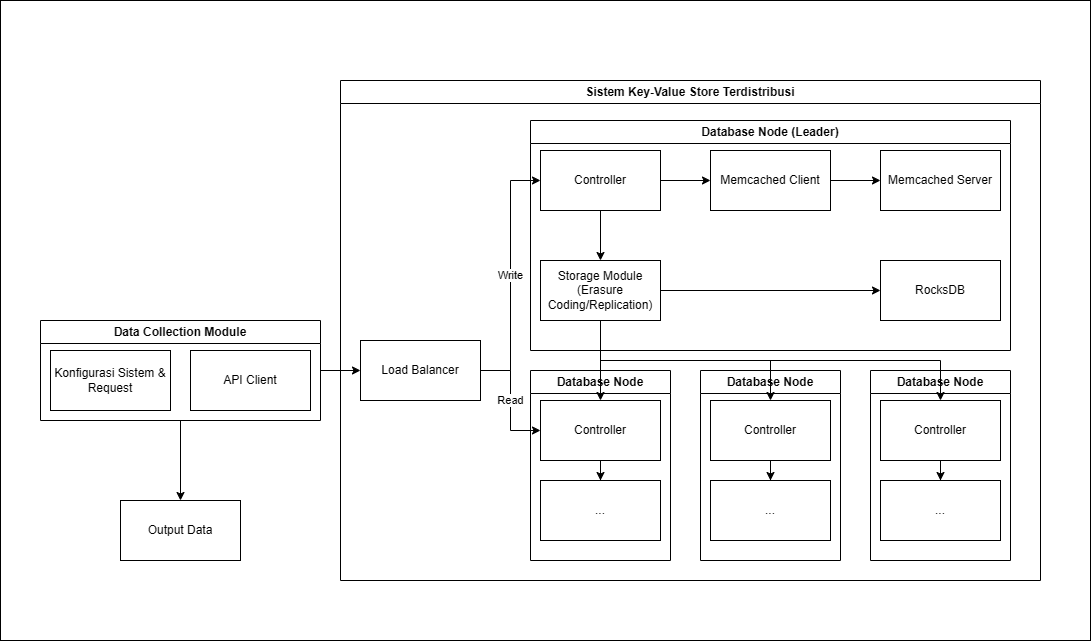
\includegraphics[width=0.75\textwidth]{resources/chapter-3/general-architecture.png}
    \caption{Gambaran Arsitektur Sistem Eksperimen}
    \label{fig:general-architecture}
\end{figure}

Dalam gambaran umum arsitektur sistem, sistem \textit{Key-Value Store} terdistribusi yang dikembangkan adalah \textit{Node}. Dalam \textit{Node} terdapat komponen penyimpanan data yang dapat diakses dan dikelola secara terdistribusi dengan dapat replikasi atau \textit{erasure coding}. Setiap \textit{Node} dapat berkomunikasi dengan \textit{Node} lainnya untuk melakukan konsensus, replikasi data, dan pemulihan data.

Sementara itu, \textit{Data collector} merupakan \textit{script} eksternal yang tidak memiliki peran dalam sistem terdistribusi, namun berfungsi untuk mengumpulkan data eksperimen. Keterhubungan \textit{Data Collector} terbatas pada komponen \textit{testing} yang dapat mengatur konfigurasi dari sistem yang akan diujikan. Detail dari masing-masing komponen akan dijelaskan pada bagian \ref{subsection:detail-komponen}. 

% Arsitektur dari sistem mengasumsikan kebutuhan untuk konsistensi yang tinggi. Untuk mencapai konsistensi tersebut, operasi \textit{write} dilakukan secara \textit{synchronous} dengan distribusi replikasi dan \textit{erasure coding} dianggap selesai ketika nilai ketahanan yang diinginkan sudah tercapai.

% Karena sistem bersifat terdistribusi, maka diperlukan sebuah algoritma konsensus untuk mengelola konsistensi antar \textit{Node}. Algoritma konsensus yang digunakan algoritma konsensus \textit{paxos} yang disesuaikan dengan kebutuhan. Salah satu penyesuaian yang dilakukan adalah mengadopsi pola \textit{leader-follower} untuk memudahkan sinkronisasi data dan mempercepat transaksi. Dengan adanya leader, fase 1 dari algoritma \textit{paxos} dapat dihilangkan dengan membuat proposal dari leader selalu memiliki nilai paling tinggi. Detail implementasi \textit{paxos} akan dijelaskan di bagian \ref{subsection:detail-komponen}. Diagram gambaran arsitektur sistem dapat dilihat pada gambar \ref{fig:general-architecture}.

% Operasi \textit{write} akan secara ekslusif disalurkan pada \textit{leader}. Kemudian untuk ketahanan, data akan didistribusikan pada \textit{follower} sesuai dengan konfigurasi \textit{node}. Sementara itu, operasi \textit{read} dapat dilakukan pada \textit{Node} manapun. Pada sistem \textit{erasure coding}, jika pada \textit{node} tersebut tidak terdapat nilai data yang dicari, maka \textit{Node} akan melakukan \textit{request} ke semua node lainnya untuk melakukan rekonstruksi data.
